\documentclass[10pt]{article}

% Packages and stuff
\usepackage[ruled,vlined]{algorithm2e}
\usepackage{algpseudocode}
\usepackage{amssymb}
\usepackage{amsmath}
\usepackage{amsthm}
\usepackage{amsfonts}
\usepackage{booktabs}
\usepackage{enumerate}
\usepackage{fancyhdr}
\usepackage{float}
\usepackage{graphicx}
\usepackage[skins]{tcolorbox}
\usepackage{mathrsfs}
\usepackage{subfig}
\usepackage[hidelinks,pdfauthor = {Maurizio M. Chiaramonte}]{hyperref}
\usepackage{bm}
\usepackage[letterpaper,margin=1in]{geometry}
\usepackage{fancyhdr}
\usepackage[explicit]{titlesec}
\usepackage{cmbright}
\renewcommand{\familydefault}{\sfdefault}

%%% Bibliography
\ifcsname#1\endcsname
\ifnum\bibliographynatbib=1
\usepackage[numbers]{natbib}
\else

\usepackage[natbib=true,maxnames=5,style=numeric,maxcitenames=1,firstinits=true,defernumbers,backend=biber,	sorting=none,
    url=false, 
    doi=false,
    eprint=false]{biblatex}
\fi
\else 
\usepackage[natbib=true,maxnames=5,style=numeric,maxcitenames=1,firstinits=true,defernumbers,backend=biber,	sorting=none,
    url=false, 
    doi=false,
    eprint=false]{biblatex}
\fi

\usepackage{multicol}
\usepackage{stmaryrd}
\usepackage{cancel}
\usepackage[utf8]{inputenc} 
\usepackage[T1]{fontenc}  
\usepackage{appendix}

%%tikz 
\usepackage{tikz}
\usetikzlibrary{arrows}
\usetikzlibrary{backgrounds}
\usetikzlibrary{calc}
\usetikzlibrary{decorations.pathmorphing}
\usetikzlibrary{decorations.pathmorphing}
\usetikzlibrary{decorations.markings}
\usetikzlibrary{decorations.pathreplacing}
\usetikzlibrary{decorations.text}

\usetikzlibrary{external}
\tikzexternalize[prefix=tikz/]
\tikzexternaldisable

\usetikzlibrary{positioning}
\usepackage{pdftexcmds}
\usetikzlibrary{positioning}
\usetikzlibrary{shapes}
\usetikzlibrary{spy}

\usetikzlibrary{knots}

\usetikzlibrary{mindmap}
\usetikzlibrary{patterns}

%% pgfplots
\usepackage{pgfplots}
\usepackage{pgffor}
\usepackage{pgfplotstable}
\pgfplotsset{compat=newest}
\usepgfplotslibrary{fillbetween}
\pgfkeys{/tikz/.cd,
  background color/.initial=white,
  background color/.get=\backcol,
  background color/.store in=\backcol,
}
\pgfplotsset{compat = newest}
\pgfplotsset{
    discard if larger/.style 2 args={
        x filter/.code={
          \edef\tempa{\thisrow{#1}}
          \edef\tempb{#2}
					\ifnum\tempa>\tempb
					\def\pgfmathresult{inf}
					\else\fi}
			}
		}
\pgfplotsset{
    discard if not/.style 2 args={
        x filter/.code={
            \edef\tempa{\thisrow{#1}}
            \edef\tempb{#2}
            \ifx\tempa\tempb
            \else
                \def\pgfmathresult{inf}
            \fi
        }
    }
}
\tikzset{
    mark position/.style args={#1(#2)}{
        postaction={
            decorate,
            decoration={
                markings,
                mark=at position #1 with \coordinate (#2);
            }
        }
    }
}
\tikzset{insert node/.style args={#1 at #2}{
    postaction=decorate,
    decoration={
      markings,
      mark= at position #2
        with
        {
         #1
        }
    }
  }
}
\usepgfplotslibrary{patchplots}



\usepackage{chngcntr}
\usepackage{etoolbox}
\usepackage{lipsum}
\newtheoremstyle{mystyle}
    {\topsep}                    % Space above
    {\topsep}                    % Space below
    {\itshape}                   % Body font
    {}                           % Indent amount
    {\scshape}                   % Theorem head font
    {.}                          % Punctuation after theorem head
    {.5em}                       % Space after theorem head
    {}  % Theorem head spec (can be left empty, meaning ‘normal’)\theoremstyle{mystyle}






\makeatletter
\providecommand*{\input@path}{}
\g@addto@macro\input@path{{./}}% append
\makeatother


\usepackage{cmbright}

% symbols
\newcommand{\rhox}{\tilde\rho}
\newcommand{\Nh}{\tilde N}

\newcommand{\xt}{{\boldsymbol x}_\top} 
\newcommand{\tipindex}{\tau}
% mathcal
\newcommand{\Ac}{\mathcal{A}}
\newcommand{\Bc}{\mathcal{B}}
\newcommand{\Cc}{\mathcal{C}}
\newcommand{\Dc}{\mathcal{D}}
\newcommand{\Ec}{\mathcal{E}}
\newcommand{\Fc}{\mathcal{F}}
\newcommand{\Gc}{\mathcal{G}}
\newcommand{\Hc}{\mathcal{H}}
\newcommand{\Ic}{\mathcal{I}}
\newcommand{\Jc}{\mathcal{J}}
\newcommand{\Lc}{\mathcal{L}}
\newcommand{\Kc}{\mathcal{K}}
\newcommand{\Mc}{\mathcal{M}}
\newcommand{\Nc}{\mathcal{N}}
\newcommand{\Oc}{\mathcal{O}}
\newcommand{\Vc}{\mathcal{V}}
\newcommand{\Pc}{\mathcal{P}}
\newcommand{\Qc}{\mathcal{Q}}
\newcommand{\qc}{\mathcal{q}}
\newcommand{\Rc}{\mathcal{R}}
\newcommand{\Sc}{\mathcal{S}}
\newcommand{\Tc}{\mathcal{T}}
\newcommand{\Wc}{\mathcal{W}}
% boldface
\newcommand{\alphab}{{\boldsymbol \alpha}}
\newcommand{\betab}{{\boldsymbol \beta}}
\newcommand{\chib}{\boldsymbol \chi}
\newcommand{\vepsb}{\boldsymbol \varepsilon}
\newcommand{\epsb}{\boldsymbol \epsilon}
\newcommand{\etab}{\boldsymbol \eta}
\newcommand{\gammab}{{\boldsymbol \gamma}}
\newcommand{\kpb}{\boldsymbol \kappa}
\newcommand{\lambdab}{{\boldsymbol \lambda}}
\newcommand{\mub}{\boldsymbol \mu}
\newcommand{\omegab}{\boldsymbol \omega}
\newcommand{\pib}{\boldsymbol \pi}
\newcommand{\psib}{\boldsymbol \psi}
\newcommand{\phib}{\boldsymbol \phi}
\newcommand{\taub}{{\boldsymbol \tau}}
\newcommand{\cs}{\boldsymbol \sigma}
\newcommand{\vphib}{\boldsymbol \varphi}
\newcommand{\xib}{{\boldsymbol \xi}}
\newcommand{\Deltab}{\boldsymbol \Delta}
\newcommand{\Omegab}{\boldsymbol \Omega}
\newcommand{\Phib}{{\boldsymbol \Phi}}
\newcommand{\Sigmab}{\boldsymbol \Sigma}
\newcommand{\Thetab}{\boldsymbol \Theta}
\newcommand{\thetab}{\boldsymbol \theta}
\newcommand{\Xib}{\boldsymbol \Xi}
\newcommand{\Pib}{\boldsymbol \Pi}

\newcommand{\1}{{\boldsymbol 1}}
\newcommand{\0}{{\boldsymbol 0}}
\newcommand{\Ab}{{\boldsymbol A}}
\newcommand{\Bb}{{\boldsymbol B}}
\newcommand{\Cb}{{\boldsymbol C}}
\newcommand{\Db}{{\boldsymbol D}}
\newcommand{\Eb}{{\boldsymbol E}}
\newcommand{\Gb}{{\boldsymbol G}}
\newcommand{\Fb}{{\boldsymbol F}}
\newcommand{\Hb}{{\boldsymbol H}}
\newcommand{\Ib}{{\boldsymbol I}}
\newcommand{\Kb}{{\boldsymbol K}}
\newcommand{\Jb}{{\boldsymbol J}}
\newcommand{\Lb}{{\boldsymbol L}}
\newcommand{\Mb}{{\boldsymbol M}}
\newcommand{\Nb}{{\boldsymbol N}}
\newcommand{\Pb}{{\boldsymbol P}}
\newcommand{\Qb}{{\boldsymbol Q}}
\newcommand{\Rb}{{\boldsymbol R}}
\newcommand{\Sb}{{\boldsymbol S}}
\newcommand{\Tb}{{\boldsymbol T}}
\newcommand{\Ub}{{\boldsymbol U}}
\newcommand{\Vb}{{\boldsymbol V}}
\newcommand{\Wb}{{\boldsymbol W}}
\newcommand{\Xb}{{\boldsymbol X}}
\newcommand{\Yb}{{\boldsymbol Y}}

\newcommand{\ab}{{\boldsymbol a}}
\newcommand{\bb}{{\boldsymbol b}}
\newcommand{\cbold}{{\boldsymbol c}}
\newcommand{\db}{{\boldsymbol d}}
\newcommand{\fb}{{\boldsymbol f}}
\newcommand{\gb}{{\boldsymbol g}}
\newcommand{\kb}{{\boldsymbol k}}
\newcommand{\hb}{{\boldsymbol h}}
\newcommand{\lb}{{\boldsymbol l}}
\newcommand{\mb}{{\boldsymbol m}}
\newcommand{\nb}{{\boldsymbol n}}
\newcommand{\pb}{{\boldsymbol p}}
\newcommand{\qb}{{\boldsymbol q}}
\newcommand{\rb}{{\boldsymbol r}}
\newcommand{\sbf}{{\boldsymbol s}}
\newcommand{\tb}{{\boldsymbol t}}
\newcommand{\ub}{{\boldsymbol u}}
\newcommand{\vb}{{\boldsymbol v}}
\newcommand{\wb}{{\boldsymbol w}}
\newcommand{\yb}{{\boldsymbol y}}
\newcommand{\zb}{{\boldsymbol z}}

\newcommand{\ti}{{\text{i}}}
\newcommand{\tj}{{\text{j}}}

% mathbb
\newcommand{\Abb}{\mathbb{A}}
\newcommand{\Ebb}{\mathbb{E}}
\newcommand{\Fbb}{\mathbb{F}}
\newcommand{\Ibb}{\mathbb{I}}
\newcommand{\Cbb}{\mathbb{C}}
\newcommand{\Jbb}{\mathbb{J}}
\newcommand{\Mbb}{\mathbb{M}}
\newcommand{\Nbb}{\mathbb{N}}
\newcommand{\Pbb}{\mathbb{P}}
\newcommand{\Qbb}{\mathbb{Q}}
\newcommand{\Rbb}{\mathbb{R}}
\newcommand{\Sbb}{\mathbb{S}}
\newcommand{\Zbb}{\mathbb{Z}}

% math sans sserif
\newcommand{\Jsf}{\mathsf{J}}

\newcommand{\jsf}{\mathsf{j}}
\newcommand{\nsf}{\mathsf{n }}
\newcommand{\rsf}{\mathsf{r}}
\newcommand{\tsf}{\mathsf{t}}

% math script
\newcommand{\Bsc}{\mathscr{B}}
\newcommand{\Csc}{\mathscr{C}}
\newcommand{\Esc}{\mathscr{E}}
\newcommand{\Fsc}{\mathscr{F}}
\newcommand{\Gsc}{\mathscr{G}}
\newcommand{\Hsc}{\mathscr{H}}
\newcommand{\Psc}{\mathscr{P}}
\newcommand{\Ssc}{\mathscr{S}}
\newcommand{\Vsc}{\mathscr{V}}
\newcommand{\Wsc}{\mathscr{W}}

% Common vectors
\newcommand{\ee}{{ \bf e}}
\newcommand{\EE}{{ \bf E}}
\newcommand{\ve}{{\boldsymbol v}}
\newcommand{\Ve}{{\boldsymbol V}}
\newcommand{\ac}{{\boldsymbol a}}
\newcommand{\x}{{\boldsymbol x}}
\newcommand{\y}{{\boldsymbol y}}
\newcommand{\X}{{\boldsymbol X}}
\newcommand{\tr}{{\bf t}}
\newcommand{\Chi}{{\boldsymbol \chi}}

\newcommand{\msp}[1]{\hbox{\hskip #1in}}
\newcommand{\mmsp}{\hbox{\hskip 0.2in}}
\newcommand{\ephi}{\,{\bf e}_{\varphi}}
\newcommand{\ff}{\,{\bf f}}
\renewcommand{\AA}{\mathbb{ A}}
\newcommand{\QQ}{\mathbb{ Q}}
\renewcommand{\SS}{\mathbb{ S}}
\newcommand{\TT}{\mathbb{ T}}
\newcommand{\ex}{\,{\bf e}_{x}}
\newcommand{\ey}{\,{\bf e}_{y}}
\newcommand{\ethe}{\,{\bf e}_{\vartheta}}
\newcommand{\dethe}{\,\dot{{\bf  e}}_{\vartheta}}
\newcommand{\dephi}{\,\dot{{\bf e}}_{\varphi}}
\newcommand{\epsi}{\,{\bf e}_{\psi}}
\newcommand{\depsi}{\,\dot{{\bf e}}_{\psi}}
\newcommand{\er}{{\,\bf e}_r}
\newcommand{\der}{\,\dot{{\bf e}}_r}
\newcommand{\dder}{\,\ddot{{\bf e}}_r}
\newcommand{\rr}{{\bf r}}

\newcommand{\nn}{{\bf n}}
\newcommand{\erdot}{(\sin(\psi)\dot{\varphi} \ephi + \dot{\psi} \epsi)}
\newcommand{\ephidot}{(-\dot{\varphi} ( \sin(\psi) \er + \cos \psi \epsi))}
\newcommand{\epsidot}{(-\dot{\psi} \er + \cos(\psi) \dot{\varphi} \ephi)}
\newcommand{\Lg}{\mathcal{L}}

% Calculus
\newcommand{\pd}[2]{ \dfrac{\partial #1}{\partial #2}}
\newcommand{\df}[2]{ \frac{d #1}{d #2}}
\newcommand{\mdf}[2]{ \frac{D #1}{D #2}}
\DeclareMathOperator{\cond}{cond}
\DeclareMathOperator{\dive}{div}
\DeclareMathOperator{\supp}{supp}
\DeclareMathOperator{\grad}{grad}
\DeclareMathOperator{\curl}{curl}
\DeclareMathOperator{\Dive}{Div}
\DeclareMathOperator{\Grad}{Grad}
\DeclareMathOperator{\Curl}{Curl}
\DeclareMathOperator{\trace}{\sf tr}
\DeclareMathOperator{\vectorspan}{span}
\DeclareMathOperator{\sign}{sign}
\DeclareMathOperator{\interior}{int}
\DeclareMathOperator{\floor}{floor}
\newcommand{\disc}[1]{\llbracket#1\rrbracket}

% Tensor Notation
\newcommand{\kd}[1]{\delta_{#1}}
\newcommand{\ten}[2]{\ee_#1\otimes\ee_#2}
\newcommand{\id}[2]{\kd{#1#2} \ee_#1\otimes\ee_#2}
\newcommand{\perm}[1]{\varepsilon_{#1}}
\DeclareMathOperator{\sym}{sym}
\DeclareMathOperator{\skews}{skew}

\newcommand{\jacobian}[2]{\mat{3}{\pd{#1_1}{#2_1} \pd{#1_1}{#2_2} \pd{#1_1}{#2_3}\\\pd{#1_2}{#2_1} \pd{#1_2}{#2_2} \pd{#1_2}{#2_3}\\\pd{#1_3}{#2_1} \pd{#1_3}{#2_2} \pd{#1_3}{#2_3}}}

% Box Answer
\newcommand{\boxeq}[1]{%
\vskip 0.5\baselineskip
\noindent\fbox{
\raggedright
\begin{minipage}[l]{\linewidth}
\vskip -0.75\baselineskip
\begin{eqnarray}
#1 
\end{eqnarray}
\end{minipage}
}
\vskip 0.5\baselineskip\noindent
}

% Equation
\newcommand{\eq}[1]{\begin{equation} #1 \end{equation}}
\newcommand{\eqnonumber}[1]{\begin{equation*} #1 \end{equation*}}
\newcommand{\eqa}[2][]{\begin{subequations}#1\begin{eqnarray} #2  \end{eqnarray}  \end{subequations}}
\newcommand{\eqas}[1]{\begin{equation}\begin{split} #1 \end{split} \end{equation}}
\newcommand{\eqax}[1]{\begin{eqnarray*} #1 \end{eqnarray*}}


\newcommand{\vect}[1]{\left\{ \begin{array}{c}#1\end{array}\right\}}
\newcommand{\mat}[2]{\left[ \begin{array}{*{#1}{c}}#2\end{array}\right]}



\newtheorem{theorem}{Theorem}[section]
\newtheorem{lemma}[theorem]{Lemma}
\newtheorem{proposition}[theorem]{Proposition}
\newtheorem{problem}[theorem]{Problem}
\newtheorem{corollary}[theorem]{Corollary}
\newtheorem{assumption}{Assumption}[section]
\usepackage{bm}



\title{homework 1}

\date{\today}

\author{APC 523: Numerical Algorithm for Scientific Computing}

\hypersetup{
	pdftitle= {\@title},
	pdfauthor = {\@author},
	pdfsubject = {},
	pdfkeywords = {},
	pdfmoddate= {\@date},
	pdfcreator = {\@author},
	pdftoolbar=true,        
	pdfmenubar=true
}



\makeatletter
\def\@maketitle{
	\begingroup
	\centering
	{
		{\Large \MakeUppercase{\@title}\par}
		\vskip 0.1\baselineskip
		{\normalsize\noindent\@author\par}
		\vskip 0.1\baselineskip
		{\normalsize\noindent Due: Oct.10\par}
	}
	\endgroup
}
\makeatother

\titleformat{\section}{\Large}{\MakeUppercase{Problem} \thesection}{1em}{\MakeUppercase{#1}}

\begin{document}

\maketitle

\section{}

Let $x=2^k(1+\sum_{i=1}^{\infty}2^{-i}b_i)$, where $k=floor(\log_2x)$

or $x=1 b_1 b_2 \cdots b_k.b_{k+1} b_{k+2}\cdots $\\

\textbf{case 1:} if $b_{p+1}=1$, then $rd(x)=2^k(1+\sum_{i=1}^{p}2^{-i}b_i+2^{-p})$

$\Rightarrow|\frac{x-rd(x)}{x}|=\frac{2^k(-2^{-p}+\sum_{i=p+1}^{\infty}2^{-i}b_i)}{2^k(1+\sum_{i=1}^{\infty}2^{-i}b_i)}\leq 2^{-p}-\sum_{i=p+1}^{\infty}2^{-i}b_i\leq2^{-p}$\\

\textbf{case 2:} if $b_{p+1}=0$, then $rd(x)=2^k(1+\sum_{i=1}^{p}2^{-i}b_i)$

$\Rightarrow|\frac{x-rd(x)}{x}|=\frac{2^k(\sum_{i=p+1}^{\infty}2^{-i}b_i)}{2^k(1+\sum_{i=1}^{\infty}2^{-i}b_i)}\leq \sum_{i=p+1}^{\infty}2^{-i}b_i\leq \sum_{i=p+1}^{\infty}2^{-i}\leq2^{-p}$\\

Therefore, $\Rightarrow|\frac{x-rd(x)}{x}|\leq2^{-p}$

\section{}

(a) The result is 244.71\\

(b) Upto $k=17$, the result does not change with 5 digits precision. The exact value is $e^{5.5}=244.692$, so relative error = $7.36(10^{-5})$\\

(c) Upto $k=17$, the result does not change with 5 digits precision, which is 244.70. The exact value is $e^{5.5}=244.692$, so relative error = $3.27(10^{-5})$\\

(d) 

\begin{tabular}{cccc}
\hline
 & \# of terms k & result & relative error ($e^{-5.5}=0.00408677$)\\
 \hline
 i & 25 & 0.038363 & 0.0613\\
 ii & 19 & 0.0040000 & 0.0212\\
 iii & 17 & 0.0000 & 1\\
 iv & 17 & 0.0000 & 1\\
 \hline
\end{tabular}

Methods iii and iv converge most quickly, but least accurate. Method ii has lowest error.

Empirically, adding from right to left is better and results in less error.\\

(e) I propose algorithm:

(i) compute $e^{0.5}$ (adding from left to right)

(ii) divide $e^{0.5}$ by $e=2.7183$ repeatedly for 6 times.\\

\underline{Validation}: result = 0.004086

relative error = $1.88(10^{-4})$

\# of terms k = 4

\section{}

(a)

(i) 

$fl(x*x)=x^2(1+\epsilon)$

$fl(x^2(1+\epsilon)*x)=x^3(1+2\epsilon)$

$\cdots$

$fl(x^{n-1}(1+(n-2)\epsilon)*x)=x^n(1+(n-1)\epsilon)$\\

(ii)

$fl(\ln x)=\ln x(1+\epsilon)$

$fl(n*ln x(1+\epsilon))=n\ln x (1+\epsilon)^2\approx n\ln x (1+2\epsilon)$

$fl(e^{n\ln x(1+2\epsilon)})=x^n e^{2\epsilon}(1+\epsilon)\approx x^n(1+3\epsilon)$

When $n-1<3$ or $n<4$, repeated multiplication is more accurate than log-exponential method.\\

(b)

(i) $x^{a(1+\epsilon_a)}=x^ax^{a\epsilon_a}=x^1e^{a\epsilon_a\ln x}\approx x^a(1+a\epsilon_a\ln x)$

(ii) $(x(1+\epsilon+x))^a=x^a(1+\epsilon_x)^a\approx x^a(1+a\epsilon_x)$

when $x\rightarrow 0,\infty$ or $|a|$ becomes large, the relative error is substantial.\\

\section{}

(a) 

$(\text{cond }f)(x)=|\frac{xf'}{f}|=\frac{x}{e^x-1}\leq 1$ because $e^x-1>x$\\

(b) 

$f_A(x)=[1-e^{-x}(1+EPS)](1+EPS)\approx (1-e^{-x})(1-\frac{e^{-x}}{1-e^{-x}}EPS)(1+EPS)\approx(1-e^{-x})(1+\frac{EPS}{1-e^{-x}})$

$f_A(x)=f(x_A)\Rightarrow |f_A(x)-f(x)|=|f(x_A)-f(x)|\approx f(x)\frac{EPS}{1-e^{-x}}\approx |f'(x)||x-x_A|$

$\Rightarrow |\frac{x-x_A}{x}|\approx|\frac{f(x)}{xf'(x)}\frac{EPS}{1-e^{-x}}|$

$\Rightarrow (\text{cond }A)(x)\approx \frac{1}{EPS}|\frac{x-x_A}{x}|\approx\frac{1}{(1-e^{-x})(\text{cond }f)(x)}=\frac{e^x}{x}$\\

(c)

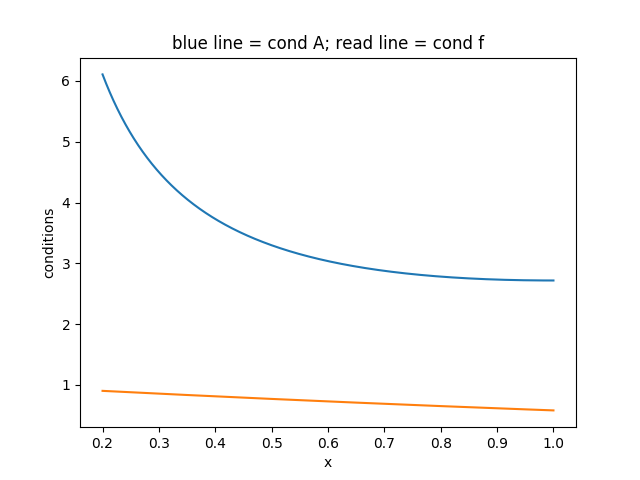
\includegraphics[width=3 in]{p4.png}

The root cause of ill conditioning is that when $x$ is small, $1-e^{-x}$ introduces a large error.\\

(d)+(e)

$1-e^{-x}<2^{-b}$ implies that less than less than $b$ bits are lost, so the minimum allowed $x$ should be

$$x=\ln(1-2^{-b})$$

In addition, the relative error should be 

$$
\epsilon=\frac{EPS}{1-e^{-x}}=2^{b}EPS
$$

\begin{tabular}{ccc}
\hline
\# bits lost & min x & relative error\\
\hline
1 & 0.693 & $2^{-51}$\\
2 & 0.288 & $2^{-50}$\\
3 & 0.134 & $2^{-49}$\\
4 & 0.0645 & $2^{-48}$\\
\hline
\end{tabular}\\

(f)

Yes, I propose the algorithm using Taylor expansion.

(i) Find $e^x-1=\sum_{n=1}^{20}\frac{x^n}{n!}$ (20 terms should be sufficiently convergent)

(ii) Find $f_A(x)=\frac{\sum_{n=1}^{20}\frac{x^n}{n!}}{1+\sum_{n=1}^{20}\frac{x^n}{n!}}$

\section{}

$n_{stop}=17$, converges to 1.

\begin{tabular}{cc}
\hline
n & result\\
\hline
n	result
$10^1$ &	2.5937424601000\\
$10^2$ &	2.7048138294215\\
$10^3$ &	2.7169239322356\\
$10^4$ &	2.7181459268249\\
$10^5$ &	2.7182682371923\\
$10^6$ &	2.7182804690958\\
$10^7$ &	2.7182816941321\\
$10^8$ &	2.7182817983474\\
$10^9$ &	2.7182820520116\\
$10^10$ &	2.7182820532348\\
$10^11$ &	2.7182820533571\\
$10^12$ &	2.7185234960372\\
$10^13$ &	2.7161100340869\\
$10^14$ &	2.7161100340870\\
$10^15$ &	3.0350352065493\\
$10^16$ &	1.0000000000000\\
$10^17$ &	1.0000000000000\\
\hline
\end{tabular}\\

This is caused by the following reasons:

\begin{enumerate}
	\item As n gets large, $(1+\frac{1}{n}(1+EPS))^n=(1+\frac{1}{n})^n(1+10n\log(n)EPS$, and the relative error will increase with n.

	\item When $n=10^{16}$, $\frac{1}{n}<EPS$, $1+\frac{1}{n}\approx 1\Rightarrow(1+\frac{1}{n})^n\approx 1 $
\end{enumerate}



\section{}

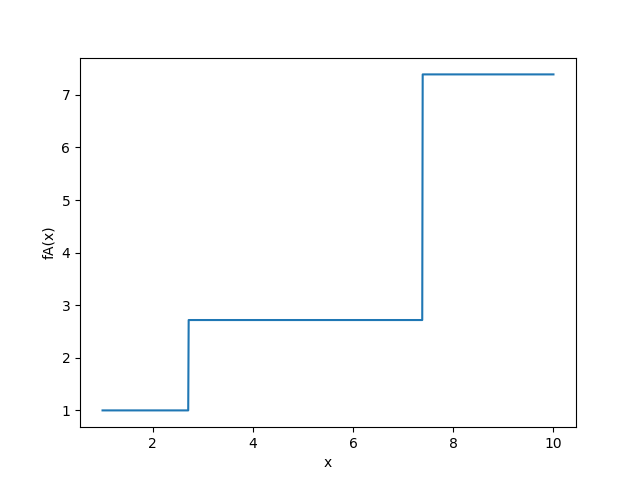
\includegraphics[width=3 in]{p6.png}

To explain this phenomenon let's define $f_1(x)=x^{2^{-52}}$, $f_2(x)=x^{2^{52}}$, such that our algorithm is $f_A(x)=f_2\circ f_1(x)=x$

Let's first look at $f_1(x)$, it can be shown that if $x=e^y$, where $e^y<<2^{52}$, then 

\begin{align*}
f_1(x)&=e^{y(2^{-52})}\\
&\approx 1+y*2^{-52}\\
&=1+y*EPS
\end{align*}

Therefore, 

if $x\in[1,e)$, $f_1(x)<1+EPS\approx 1\Rightarrow f_A(x)=1$;

if $x\in[e,e^2)$, $f_1(x)\in[1+EPS,1+2*EPS)\approx 1+EPS\Rightarrow f_A(x)=(1+EPS)^{2^{52}}$;

if $x\in[e^2,e^3)$, $f_1(x)\in[1+2*EPS,1+3*EPS)\approx 1+2*EPS\Rightarrow f_A(x)=(1+2*EPS)^{2^{52}}$



\section{}

(a)

$w(x) = x^{20} -210x^{19}+                20615x^{18}
-1256850x^{17}             +53327946x^{16}          -1672280820x^{15}
+40171771630x^{14}        -756111184500x^{13}       +11310276995381x^{12}
-135585182899530x^{11}     +1307535010540395x^{10}   -10142299865511450x^9
+63030812099294896x^8  -311333643161390640x^7  +1206647803780373360x^6
-3599979517947607200x^5  +8037811822645051776x^4  +5575812828558562816x^3
-4642984320068847616x^2 -8752948036761600000x  +2432902008176640000$\\

(b)

root = 19.99987405572419\\

(c)

\begin{tabular}{cc}
	\hline
$\delta$ & max root\\
\hline
$10^{-8}$ & (20.647582887998496+1.1869261883090942j)\\
$10^{-6}$ & (23.149016020150878+2.740984637982632j)\\
$10^{-4}$ & (28.40021241591655+6.5104342165628175j)\\
$10^{-2}$ & (38.478183617151515+20.83432358712749j)\\
\hline
\end{tabular}\\

(d) Let $a_{19}=-210-2^{-23}$, roots 16, 17 become 16.73074488+2.8126249j, 16.73074488-2.8126249j\\


(e)

(i) To find $(\text{cond } \Omega_k)(\vec{a})$, let's impose a perturbation on $a_l$, such that $a_l(1+\epsilon_l)$ results in a new root $\Omega_k(1+\epsilon_k)$

By definition, $a_0+a_1\Omega_k+\cdots a_n\Omega_k^n=0$. In addition, after perturbation, we have

\begin{align*}
0&=a_0+a_1\Omega_k(1+\epsilon_k)+\cdots +a_l(1+\epsilon_l)\Omega_k^l(1+\epsilon_k)^l+\cdots + a_n\Omega_k^n(1+\epsilon_k)^n\\
& = a_1\Omega_k(\epsilon_k)+a_2\Omega_k^2(2\epsilon_k) +\cdots +a_l\Omega_k^l(l\epsilon_k+\epsilon_l)+\cdots a_n\Omega_k^n(n\epsilon_k)\\
&=p'(\Omega_k)\Omega_k\epsilon_k+a_l\Omega_k^l\epsilon_l\\
\Rightarrow \Gamma_{kl}&=|\frac{\epsilon_k}{\epsilon_l}|=|\frac{a_l\Omega_k^l}{p'(\Omega_k)\Omega_k}|
\end{align*}

Therefore,
$$
(\text{cond } \Omega_k)(\vec{a})=\sum_{l=0}^{n}|\frac{a_l\Omega_k^l}{p'(\Omega_k)\Omega_k}|
$$

(ii)

\begin{tabular}{cc}
\hline
$\Omega_k$ & $(\text{cond } \Omega_k)(\vec{a})$\\
\hline
14 & 251350894804.7394\\
16 & 104194884779.65079\\
17 & 71181306412.37926\\
20 & 35518935656.3619\\
\hline
\end{tabular}\\

(iii)

There is no smart algorithm because the problem is by nature ill-conditioned.

\section{}

(a) 

Use the recurrence relation $y_{n-1}=\frac{e-y_n}{n}$

$y_{k-1}=\frac{e-y_k(1+\epsilon_k)}{k}=\frac{e-y_k}{k}(1+\frac{y_k}{e-y_k}\epsilon_k)$

$\Rightarrow \epsilon_{k-1}=\frac{y_k}{e-y_k}\epsilon_k$\\

\underline{Estimation of Upper Bound:}

$y_k\leq\int_{0}^{1}ex^kdx=\frac{e}{k+1}\Rightarrow \epsilon_{k-1}\leq\frac{\frac{e}{k+1}}{e-\frac{e}{k+1}}=\frac{1}{k}\epsilon_k$

$\Rightarrow \epsilon_k\leq(\frac{1}{k})^{N-k}\epsilon_N$

$\Rightarrow (\text{cond }g_k)(y_N)\leq(\frac{1}{k})^{N-k}$\\

(b)

$\epsilon_N=1\Rightarrow \epsilon_k\leq(\frac{1}{k})^{N-k}\epsilon_N=(\frac{1}{k})^{N-k}$

$\Rightarrow N\geq k+\log_k(1/\epsilon)$\\

(c)

$\epsilon=EPA=2.2(10^{-16}) \Rightarrow N=20-\log_{20}(2.2)+16\log_{20}(10)=32.03\approx 33$\\

(d)

From Wolfram : $y_{20}=0.12380$

$N=33\Rightarrow y_{20}=0.12380$, so the result can be verified.





\end{document}